\documentclass[10pt,openany]{book}
\usepackage[utf8]{inputenc}
\usepackage[T1]{fontenc}
\usepackage[dvips,a4paper,hmargin={4cm,4cm},vmargin={3.5cm,3.5cm}]{geometry}
\usepackage[a4paper,colorlinks=true,bookmarksopen=false,linkcolor=brown,citecolor=red]{hyperref}
\usepackage{pythontex}
\usepackage{calc}
\usepackage{comment}
\usepackage{amssymb}
\usepackage{amsthm}
\usepackage{amsmath}
\usepackage{amsrefs}
\usepackage{titlesec}
\usepackage{titletoc}
\usepackage{dsfont}
\usepackage{euscript}
\usepackage{fourier-orns}
\usepackage{fontawesome}
\usepackage{palatino}
\usepackage{graphicx}
\usepackage{tikz-cd}
\tikzcdset{
arrow style=tikz,
diagrams={>=latex}
}

\def\RR{\mathds R}
\def\ZZ{\mathds Z}
\def\NN{\mathds N}
\def\QQ{\mathds Q}
\def\P{\EuScript P}
\def\0{\varnothing}
\def\E{{\rm E}}
\def\Var{{\rm Var}}
\def\range{\mathop{\rm img}}
\def\H0{{\rm H_0}}
\def\HA{{\rm H_A}}

\linespread{1.2}
\setlength{\parindent}{0ex}
\setlength{\parskip}{.5\baselineskip}

% \DeclareFontFamily{OT1}{pzc}{}
% \DeclareFontShape{OT1}{pzc}{m}{it}{<-> s * [1.10] pzcmi7t}{}
% \DeclareMathAlphabet{\mathpzc}{OT1}{pzc}{m}{it} 


\newcommand{\mylabel}[1]{{\footnotesize\textsf{#1}}\hfill}
\renewenvironment{itemize}
  {\begin{list}{$\triangleright$}{%
   \setlength{\parskip}{0mm}
   \setlength{\topsep}{.2\baselineskip}
   \setlength{\rightmargin}{0mm}
   \setlength{\listparindent}{0mm}
   \setlength{\itemindent}{0mm}
   \setlength{\labelwidth}{3ex}
   \setlength{\itemsep}{.4\baselineskip}
   \setlength{\parsep}{0mm}
   \setlength{\partopsep}{0mm}
   \setlength{\labelsep}{1ex}
   \setlength{\leftmargin}{\labelwidth+\labelsep}
   \let\makelabel\mylabel}}{%
   \end{list}\vspace*{-1.3mm}}

   
\definecolor{blue}{rgb}{0, 0.1, 0.6}
\def\emph#1{\textcolor{blue}{\textbf{\boldmath #1}}}

\def\theta{\vartheta}
\def\phi{\varphi}
\def\epsilon{\varepsilon}
\def\ssf#1{\textsf{\small #1}}

\titlecontents{section}
[3.8em] % ie, 1.5em (chapter) + 2.3em
{\vskip-1ex}
{\contentslabel{1.5em}}
{\hspace*{-2.3em}}
{\titlerule*[1pc]{}\contentspage}


\titleformat
{\chapter} % command
[display] % shape
{\bfseries\LARGE} % format
{Chapter \ \thechapter} % label
{0.5ex} % sep
{} % before-code
[] % after-code
\titleformat{\section}[block]{\Large\bfseries}{\makebox[5ex][r]{\textbf{\thesection}}}{1.5ex}{}
\titlespacing*{\chapter}{0em}{.5ex plus .2ex minus .2ex}{2.3ex plus .2ex}
\titlespacing*{\section}{-9.7ex}{3ex plus .5ex minus .5ex}{1ex plus .2ex minus .2ex}

\renewcommand*\thesection{\arabic{section}}

\newtheoremstyle{mio}% name
     {2\parskip}%      Space above
     {\parskip}%      Space below
     {\sl}%         Body font
     {}%         Indent amount (empty = no indent, \parindent = para indent)
     {\bfseries}% Thm head font
     {}%        Punctuation after thm head
     {1.5ex}%     Space after thm head: " " = normal interword space;
           %   \newline = linebreak
     {\llap{\thmnumber{#2}\hskip2mm}\thmname{#1}\thmnote{\bfseries{} #3}}% Thm head spec (can be left empty, meaning `normal')

\newtheoremstyle{liscio}% name
     {2\parskip}%      Space above
     {0mm}%      Space below
     {}%         Body font
     {}%         Indent amount (empty = no indent, \parindent = para indent)
     {\bfseries}% Thm head font
     {}%        Punctuation after thm head
     {1.5ex}%     Space after thm head: " " = normal interword space;
           %   \newline = linebreak
     {\llap{\thmnumber{#2}\hskip2mm}\thmname{#1}\thmnote{\bfseries{} #3}}% Thm head spec (can be left empty, meaning `normal')

\newcounter{thm}[chapter]

\renewcommand{\thethm}{\thechapter.\arabic{thm}}

\theoremstyle{mio}
\newtheorem{theorem}[thm]{Theorem}
\newtheorem{corollary}[thm]{Corollary}
\newtheorem{proposition}[thm]{Proposition}
\newtheorem{lemma}[thm]{Lemma}
\newtheorem{fact}[thm]{Fact}
\newtheorem{void_thm}[thm]{}
\newtheorem{definition}[thm]{Definition}
\theoremstyle{liscio}
\newtheorem{void_def}[thm]{}
\newtheorem{remark}[thm]{Remark}
\newtheorem{notation}[thm]{Notation}
\newtheorem{note}[thm]{Note}
\newtheorem{exercise}[thm]{Exercise}
\newtheorem{example}[thm]{Example}
\setlength{\partopsep}{0mm}
\setlength{\topsep}{0mm}
\def\QED{\noindent\nolinebreak[4]\hfill\rlap{\ \ $\Box$}\medskip}
\renewenvironment{proof}[1][Proof]%
{\begin{trivlist}\item[\hskip\labelsep {\bf #1}]}
{\QED\end{trivlist}}

\newenvironment{void}[1][]%
{\begin{trivlist}\item[\hskip\labelsep {\bf #1}]}
{\QED\end{trivlist}}



\pagestyle{empty}

\definecolor{violet}{RGB}{115, 0, 205}
\definecolor{brown}{RGB}{150, 50, 10}
\definecolor{green}{RGB}{10,120, 20}
\def\mr{\color{brown}}
\def\gr{\color{green}}
\def\vl{\color{violet}}



\begin{document}
\setlength{\abovedisplayskip}{-1ex}
\setlength{\belowdisplayskip}{0pt}




\chapter{Teoria (il minimo sindacale)}
\raggedbottom

Per esempi e esercizi seguire i \hyperref[ch2]{link \faShare}


%%%%%%%%%%%%
%%%%%%%%%%%%
%%%%%%%%%%%%
\clearpage\section{Variabili aleatorie}


\def\medrel#1{\parbox[t]{6ex}{$\displaystyle\hfil #1$}}
\def\ceq#1#2#3{\parbox{25ex}{$\displaystyle #1$}\medrel{#2}$\displaystyle  #3$}


Fisssiamo un insieme non vuoto \emph{$\Omega$\/} che chiameremo \emph{spazio campionario\/}  (\emph{sample space\/}) o \emph{popolazione}. Immagimiamo gli elementi \emph{$\omega$\ }$\in\Omega$ come i possibili \emph{risultati\/} di un rilevamento, un esperimento, un sorteggio, ecc. I sottoinsiemi $E\subseteq\Omega$ verranno chiamati \emph{eventi\/} e rapresentano proprietà osservabili.

Una \emph{misura di probabilità\/} è una funzione $P:\P(\Omega)\to\RR$ tale che 

\begin{itemize}
\item $P(\Omega)=1$
\item $P(A)\ge0$ per ogni $A\in\P(\Omega)$
\item $P(A\cup B)=P(A)+P(B)$ per ogni coppia $A,B\in\P(\Omega)$ di insiemi \emph{disgiunti}, ovvero $A\cap B=\0$. Si dice anche che $A$ e $B$ sono \emph{mutualmente esclusivi}.
\end{itemize}

Sia $R$ un insieme quasiasi. Una \emph{variabile aleatoria\/} è una funzione $X:\Omega\to R$. Se $R$ è un insieme numerico (un sottoinsieme di $\NN$, $\ZZ$, $\QQ$, $\RR$, $\RR^2$, ecc.) diremo che $X$ è una \emph{variabile aleatoria numerica}. Una variabile aleatoria non numerica è detta \emph{qualitativa\/} o \emph{categorica}.


%%%%%%%%%%%%
%%%%%%%%%%%%
%%%%%%%%%%%%
\clearpage\section{Distribuzione di probabilità discreta}

Come sopra $X:\Omega\to R$ è una variabile aleatoria. Dato $x\in R$ e $A\subseteq R$ scriveremo

\ceq{\hfill \emph{$p_x$}\medrel{=}\emph{$P(X=x)$}}{=}{P\big(\{\omega\in\Omega\ :\ X(\omega)=x)\}\big)}

\ceq{\hfill \emph{$P(X\in A)$}}{=}{P\big(\{\omega\in\Omega\ :\ X(\omega)\in A)\}\big)}

\ceq{\hfill \emph{$P(X \le x$)}}{=}{P\big(\{\omega\in\Omega\ :\ X(\omega)\le x)\}\big)}\hfill  se $X$ \`e numerica.

La funzione $P(X=x)$ si chiama \emph{distribuzione di probabilità discreta (probability mass function)}. La funzione $P(X \le x)$ si chiama  \emph{funzione di ripartizione (cumulative distribution function)}.

Le variabili numeriche possono dirsi \emph{discrete\/} o \emph{continue}. Una v.a.\@ $X$ è discreta se per ogni sottoinsieme $A\subseteq R$

\ceq{\hfill P\big(X\in A\big)}{=}{\sum_{x\in A}P(X=x)}

Ovvero la probabilità è concentrata nei punti di $R$. Invece una variabile continua se $P(X=x)=0$ per ogni $x\in R$. Per le variabili continue tutta l'informazione è contenuta nella funzione di ripartizione possiamo solo scrivere


\ceq{\hfill P\big(X\in [a,b]\big)}{=}{P(a \le X \le b)\medrel{=}P(X\le b)-P(X\le a)}

Si noti che la seconda uguaglianza non sarebbe corretta se $P(X=a)\neq0$.

N.B. Esistono variabili aleatorie (anche in esempi concreti) che sono intermedie tra il continuo e il discreto ma per il momento non le considereremo.



%%%%%%%%%%%%
%%%%%%%%%%%%
%%%%%%%%%%%%
\clearpage\section{Variabili aleatorie di Bernoulli}

Una variabile aleatoria $X$ si dice di bernulli se \emph{Bernoulli\/} se $\range X=\{0,1\}$.

Possiamo identificare in modo canonico eventi e variabili aletorie di Bernoulli. L'evento associato ad $X$ è l'insieme $\{\omega:X(\omega)=1\}$ che chiameremo \emph{successo}. Chiameremo \emph{$p$}\ $ = P(X=1)$ la \emph{propbabilità di successo}.

Viceversa, la v.a.\@ di Bernoulli associata ad un evento $E$ è spesso denotata con $1_E$

\ceq{\hfill 1_E(x)}{=}{\left\{\begin{array}{ll}1&\textrm{ se }\ x\in E\\0&\textrm{ se }\ x\notin E\end{array}\right.}

Per dire che $X$ è una variabile aleatoria di Bernoulli con probabilità di successo $p$ scriveremo \emph{$X\sim B(1,p)$}.



%%%%%%%%%%%%
%%%%%%%%%%%%
%%%%%%%%%%%%
%%%%%%%%%%%%
\clearpage\section{Probabilità condizionata} 

{\color{brown}Esempi:} \hyperref[MF_totali]{Popolazione maschile e femminile (probabilità totali) \faShare}
\\
\hphantom{Esempi:} \hyperref[Fumatori_Bayes]{Fumatori (regola di Bayes) \faShare}
\\
\hphantom{Esempi:} \hyperref[rain_desert]{Rain forcasts (Bayes rule) \faShare}


Dato $A, \Phi\subseteq\Omega$ tali che $P(\Phi)\neq 0$ definiamo 

\ceq{\hfill \emph{$P(A\mathbin|\Phi)$}}{=}$\displaystyle\frac{P(A\cap\Phi)}{P(\Phi)\vphantom{\Big[}}$

Questo si legge \emph{probabilità di $A$ dato $\Phi$}. Si verifica facilmente che $P(\,\cdot\,|\Phi)$ soddisfa a tutte le propriet\`a di $P(\,\cdot\,$) se rimpiazziamo $\Omega$ con $\Phi$.

Il fatto seguente si chiama \emph{Teorema delle Probabilità Totali}. Siano $A_1,\dots,A_n$ eventi \emph{mutuamente esclusivi\/} ed \emph{esaustivi} di probabilità $\neq0$. Sia $C$ \`e un qualsiasi altro evento, allora

\ceq{\hfill P(C)}{=}{\sum^n_{i=1} P(A_i)\cdot P\big(C| A_i).}

Il seguente di chiama \emph{Teorema (o regola) di Bayes}. Per ogni coppia di eventi $A$ e $B$ di probabilit\`a $\neq0$ 

\ceq{\hfill P(A|B)}{=}{\frac{P(B|A)\cdot P(A)}{P(B)\vphantom{\Big[}}}

In molte applicazioni $P(B)$ viene calcolato usanto il teorema delle probabilità totali.

\ceq{}{=}{\frac{P(B|A)\cdot P(A)}{P(B|A)P(A)+P(B|\neg A)P(\neg A)\vphantom{\Big[}}}


%%%%%%%%%%%%%%%%%%%%%%%
%%%%%%%%%%%%%%%%%%%%%%%
%%%%%%%%%%%%%%%%%%%%%%%
%%%%%%%%%%%%%%%%%%%%%%%
\clearpage\section{Indipensenza stocastica}

Due eventi $A$ e $B$ si dicono \emph{(stocasticamente) indipenenti\/} se 

\ceq{\hfill P(A\cap B)}{=}{P(A)\cdot P(B)}. 

Il seguente fatto è facile da verificare: se $A$ e $B$ sono eventi probabilità non nulla allora sono indipendenti se e solo se $P(A|B)=P(A)$ se e solo se $P(B|A)=P(B)$.

Due variabili aleatorie discrete $X$ ed $Y$ si dicono \emph{(stocasticamente) indipenenti\/} se per ogni $x\in\range X$ e $y\in\range Y$

\ceq{\hfill P(X, Y =x,y)}{=}{P(X=x)\cdot P(Y=y)}.

Nel caso di variabili aleatorie continue la condizione diventa


\ceq{\hfill P(X\le x\ \textrm{ and }\ Y\le y)}{=}{P(X\le x)\cdot P(Y\le y)}.



%%%%%%%%%%%%%%%%%%%%%%%
%%%%%%%%%%%%%%%%%%%%%%%
%%%%%%%%%%%%%%%%%%%%%%%
%%%%%%%%%%%%%%%%%%%%%%%
\clearpage\section{Esperimenti ripetuti: prodotto di spazi di probabilità}

Sia $X:\Omega\to\{0,1\}$ una variabile aleatoria di Bernoulli (per avere un esempio semplice). Immaginiamo che $X$ modelli il lancio di una moneta. Per brevità scriviamo $A$ per $X^{-1}[\,1\,]$.

Il lancio ripetuto di una monetina è modellato con lo spazio campionario $\Omega^2$. L'insieme  $A\times\Omega$ è l'evento dello spazio $\Omega^2$ che corrisponde  ad ottenere $1$ nel primo lancio. L'insieme $\Omega\times\neg A$ corrisponde ad ottenere $0$ nel secondo lancio.

L'intersezione di questi eventi è $A\times\neg A$. Questo corrisponde ad ottenere nei due lanci la sequenza $1\,0$. 

La probabilità di un evento $A\times B\subseteq\Omega^2$ è per definizione $P(A)\cdot P(B)$. Gli eventi $A\times\Omega$ e $\Omega\times B$ sono quindi indipendenti.




%%%%%%%%%%%%%%%%%%%%%%%
%%%%%%%%%%%%%%%%%%%%%%%
%%%%%%%%%%%%%%%%%%%%%%%
%%%%%%%%%%%%%%%%%%%%%%%
\clearpage\section{Variabili aleatorie binomiali}






%%%%%%%%%%%%%%%%%%%%%%%
%%%%%%%%%%%%%%%%%%%%%%%
%%%%%%%%%%%%%%%%%%%%%%%
%%%%%%%%%%%%%%%%%%%%%%%
\clearpage\section{Valore atteso e varianza}

Il \emph{valore atteso\/} o \emph{media di popolazione\/} (\emph{expected value, population mean\/}) di una variabile aleatoria numerica discreta $X$ a valori in $R$ è

\ceq{\hfill\emph{$\mu\medrel{=} \E(X)$}}{=}{\sum_{x\in R} x\cdot P(X=x)}

La \emph{varianza\/} di una variabile aleatoria numerica discreta $X$ a valori in $R$ è

\ceq{\hfill\emph{$\sigma^2\medrel{=} \Var(X)$}}{=}{\sum_{x\in R} \big(x- E(X)\big)^2\cdot P(X=x)}

\ceq{}{=}{E(X^2)-E(X)^2}\hfill (facile da verificare).

La \emph{deviazione standard\/} è la radice della varianza

\ceq{\hfill \emph{$\sigma$}}{=}{\sqrt{\Var(X)\vphantom{\big[]}}}

Le lettere $\mu$ e $\sigma$ vengono usate quando è chiaro a quale variabile ci si riferisce. per evitare ambiguità a volte si scrive $\mu_X$ e $\sigma_X$.




%%%%%%%%%%%%
%%%%%%%%%%%%
%%%%%%%%%%%%
\clearpage\section{Diagnostic tests}


{\color{brown}Esempi:}  \hyperref[HIV_test]{HIV test (regola di Bayes) \faShare}
% \\
% \hphantom{Esempi:}

Let \emph{$T_+$\/} and \emph{$T_-$\/} be the events that the result of a diagnostic test
is positive or negative respectively. Let \emph{$D$\/} be the event that the subject of the test has the disease. 

Introduciamo un po di terminologia.

\begin{itemize}
\item We call $P(D)$ the \emph{prevalence\/} of the disease. Often it is very difficult to estimate: it strongly depends on the risk category the subject belongs to.
\item The \emph{sensitivity\/} is the probability that the test is
positive given that the subject actually has the disease, $P(T_+ | D)$
\item The \emph{specificity\/} is the probability that the test is
negative given that the subject does not have the disease, $P(T_- | \neg D)$
\item The \emph{positive predictive value\/} is the probability that the subject has the
disease given that the test is positive, $P(D | T_+)$
\item The \emph{negative predictive value\/} is the probability that the subject does not have
the disease given that the test is negative, $P(\neg D | T_-)$
\item The \emph{prevalence of the disease\/} is the marginal probability of disease, $P(D)$

\end{itemize}


Tipicamente la specificità e la sensitività del test sono note. I poteri predittivi positivi e negativi vengono calcolati usando la prevalenza e regola di Bayes e quindi dipendono fortemente dalla categoria di rischio del cui appartiene il soggetto.





%%%%%%%%%%%%
%%%%%%%%%%%%
%%%%%%%%%%%%
\clearpage\section{Campioni e statistiche}

Un campione $\{X_1,\dots,X_n\}$ è un insieme di $n$ v.a.\@ indipendenti e identicamente distribuite. Diremo che il campione ha \emph{rango\/} (o \emph{dimensione\/}) $n$. 

Una \emph{statistica\/} è una variabile aleatoria a valori in $\RR$ ottenuta come funzione delle variabili aleatorie di un campione. Gli esempi più noti sono $\bar X$, la \emph{media campionaria\/} ed $S$, lo \emph{stimatore della deviazione standard\/} 

\ceq{\hfill \emph{$\bar X$}}{=}{\frac1n\sum_{i=1}^n X_i}

\ceq{\hfill  \emph{$S$}}{=}{\sqrt{\frac1{n-1}\sum_{i=1}^n (X_i-\bar X)^2}}
 




%%%%%%%%%%%%
%%%%%%%%%%%%
%%%%%%%%%%%%
\clearpage\section{Test d'ipotesi}

Esempi: \hyperref[Bernoulli_test]{Bernoulli test (il più elementare test di ipotesi) \faShare}

Nei test di ipotesi la scelta tra risultato positivo/negativo viene fatta in base al valore di una statistica. Si sceglie un intervallo detto \emph{regione di rifiuto\/}. Se il valore è in questo intervallo l'esito si considera positivo (N.B.\@ rifiuto$\,\sim\,$positivo).

Introduciamo la terminologia dei test d'ipotesi basandoci sulla notazione usata per i test diagnostici.

\begin{itemize}
\item L'\emph{ipotesi nulla\/} denotata con \emph{$\H0$} definisce l'insieme dei \textit{sani\/} (qui denotato $\neg D$). 
\item L'\emph{ipotesi alternativa\/} denotata con \emph{$\HA$}  descrive la \textit{patologia}, ovvero definisce l'insieme dei \textit{malati\/} (qui denotato  $D$).

\item $\HA$ non è semplicemente la negazione di $\H0$. Alcune possibilità potrebbero non occorrere né in $\H0$ né in $\HA$ perché ritenute impossibili.

\item L'espressione: \emph{$\H0$ può essere rifiutata\/} è sinonima di \textit{l'esito del test è positivo}. 
Noi denotiamo l'evento con $T_+$.


\item L'espressione: \emph{$\H0$ NON può essere rifiutata\/} è sinonima di \textit{l'esito del test è negativo}. 
Noi denotiamo l'evento con $T_-$.

\item Nel progettare il test si decide come definire $T_+$ e $T_-$ a seconda di quanti falsi positivi/negativi si vuole o può tollerare (in base ai costi/rischi che questi due errori comportano). Ci si calcola quindi $P(T_+|\neg D)$ e $P(T_-| D)$.
\end{itemize}

N.B. È vacile progettare un test che minimizza solo una tra $P(T_+|\neg D)$ o $P(T_-| D)$. In un caso estremo: un test che a prescindere dai dati rifiuta sempre $\H0$ avrà banalmente $P(T_-| D)=0$; invece un test che non rifiuta mai $\H0$ avrà  $P(T_+|\neg D)=0$.

La difficoltà nel progettare il test è trovare il giusto equilibrio tra $P(T_+|\neg D)$ e $P(T_-| D)$.



%%%%%%%%%%%%
%%%%%%%%%%%%
%%%%%%%%%%%%
\clearpage\section{Test d'ipotesi (tavola riassuntiva)}
\setlength{\fboxsep}{1.2ex}

Evidenziamo in questa tavola la terminologia usata nei test statistici (che differisce da quella usata per i test diagnostici). Molto comune sono i simboli $\emph{$\alpha$\/}=P(T_+|\neg D)$ e $\emph{$\beta$\/}=P(T_-| D)$.\bigskip   


\fbox{\parbox[t]{34ex}{%
$T_+\cap \neg D$ \ falso pos.\hfill \emph{errore I tipo\/}\\

$P(T_+|\neg D)=\emph{$\alpha$}$\hfill \emph{significatività\/}
}}
\kern2ex
\fbox{\parbox[t]{36ex}{%
$T_+\cap D$ \ corretto pos.\\

$P(T_+| D)=1-\emph{$\beta$}$ \ sensibilità\hfill \emph{potenza\/}
}}


\fbox{\parbox[t]{34ex}{%
$T_-\cap\neg D$ \ corretto neg.\\

$P(T_-|\neg D)=1-\emph{$\alpha$}$\hfill \emph{sepecificità\/}
}}
\kern2ex
\fbox{\parbox[t]{36ex}{%
$T_-\cap D$ \ falso neg.\hfill \emph{errore II tipo\/}\\

$P(T_-| D)=\emph{$\beta$}$
}}

%%%%%%%%%%%%
%%%%%%%%%%%%
%%%%%%%%%%%%
\clearpage\section{Il p-valore}






\chapter{Esempi ed esercizi}
\label{ch2}

\ \ 



%%%%%%%%%%%%
%%%%%%%%%%%%
%%%%%%%%%%%%
\clearpage\section{Pobabilità totali: maschi e femmine}
\label{MF_totali}




%%%%%%%%%%%%
%%%%%%%%%%%%
%%%%%%%%%%%%
\clearpage\section{Regola di Bayes: fumatori e non fumatori}
\label{Fumatori_Bayes}



%%%%%%%%%%%%
%%%%%%%%%%%%
%%%%%%%%%%%%
\clearpage\section{Bayes rule: Rain forcasts}
\label{rain_desert}

Marie is getting married tomorrow at an outdoor ceremony in the desert. In recent years it has rained only $5$ days each year. But the weatherman has predicted rain for tomorrow. When it actually rains, the weatherman correctly forecasts rain $90\%$ of the time. When it doesn’t rain, he incorrectly forecasts rain $10\%$ of the times. What is the probability that it will rain on the day of Marie’s wedding?


$R$\hfill event: it rains on Marie’s wedding

$T_+$\hfill event: the weatherman predicts rain

$P (R) = 5/365$\hfill it rains 5 days out of the year

$P (\neg R) = 1-P(R)= 360/365$

$P (T_+|R) = 0.9$\hfill when it rains, $90\%$ of the times rain is predicted

$P (T_+|\neg R) = 0.1$\hfill when it does not rain, $10\%$ of the times rain is predicted

\bigskip
We want to know

$\displaystyle P(R\,| T_+)\medrel{=}\frac{P(R)\cdot P(T_+|R)}{P(T_+)\vphantom{\Big[}}$

$\displaystyle\hphantom{P(R | T_+)}\medrel{=}\frac{P(R)\cdot P(T_+|R)}{P(T_+|R)\cdot P(R)+ P(T_+|\neg R)\cdot P(\neg R)\vphantom{\Big[}}$


%%%%%%%%%%%%
%%%%%%%%%%%%
%%%%%%%%%%%%
\clearpage\section{Indipendenza}
\label{esercizio_indipendenza}

Lanciamo una moneta $2n$ volte. Modelliamo l'esperimento con una sequenza $X_0,\dots,X_{2n-1}$ di variabili di Bernoulli. N.B.\@ cominciamo ad enumerare da $0$. Dire quali delle seguenti coppie di variabili aleatorie $X$, $Y$ sono indipendenti.\medskip

\begin{itemize}
\item[1.] $\displaystyle X=\sum_{i=0}^{n-1}X_i$\qquad $\displaystyle Y=\sum_{i=n}^{2n-1}X_i$.


\item[2.] $\displaystyle X=\sum_{i=0}^{n}X_{2i}$\qquad $\displaystyle Y=\sum_{i=0}^{i} X_{2i-1}$.\bigskip

\item[3.] $X= \#\big\{i<n\ |\ X_{2i}\neq X_{2i+1}\big\}$;\\
$Y= \#\big\{i<n\ |\ X_{2i+1}\neq X_{2i}\big\}$.\bigskip

\item[4.] $X=0$ se $X_0\neq X_1$ altrimenti $=1$. \\
$Y=0$ se $X_1\neq X_2$, altrimenti $=1$.

\end{itemize}



%%%%%%%%%%%%
%%%%%%%%%%%%
%%%%%%%%%%%%
\clearpage\section{Diagnostic test: HIV}
\label{HIV_test}

A study comparing the efficacy of HIV tests, reports on an
experiment which concluded that HIV antibody tests have a
{\color{brown}sensitivity of 99.7\%} and a {\color{brown}specificity of 98.5\%}

Suppose that a subject, from a population with a {\color{brown} 0.1\% prevalence}
of HIV, receives a positive test result. What is the probability
that this subject has HIV?

Mathematically, we want $P(D | T_+)$ given the sensitivity, {\color{brown}$P(T_+
| D) = .997$}, the specificity, {\color{brown}$P(T_- | \neg D) =.985$}, and the
prevalence {\color{brown}$P(D) = .001$}

\begin{eqnarray*}
P(D ~|~ +)& = &\frac{P(T_+|D)P(D)}{P(T_+)\vphantom{\Big[}}\\ \\
& = &\frac{P(T_+|D)P(D)}{P(T_+|D)\ P(D) + P(T_+|\neg D)\ P(\neg D)\vphantom{\Big[}}\\ \\
& = & \frac{P(T_+|D)P(D)}{P(T_+|D)P(D) + \big[1-P(T_-|\neg D)\big]\ \big[1 - P(D)\big]\vphantom{\Big[}} \\ \\
%& = & \frac{.997\times .001}{.997 \times .001 + .015 \times .999}\\ \\
& = & 0.062
\end{eqnarray*}

The {\color{brown}positive predictive value is 6\%} for this test. In this population a positive test result only suggests a 6\% probability that the subject has the disease. 


The low positive predictive value is due to low prevalence of disease and the
somewhat modest specificity 

Suppose it was known that the subject was an intravenous drug user and routinely had intercourse with an HIV infected partner that the test was taken in South Africa where the prevalence is estimated to be around 20\%

\begin{eqnarray*}
P(D ~|~ +)& = & 0.943\\
& \hphantom{=} & \hphantom{\frac{P(T_+|D)P(D)}{P(T_+|D)P(D) + \big[1-P(T_-|\neg D)\big]\ \big[1 - P(D)\big]\vphantom{\Big[}}}
\end{eqnarray*}



%%%%%%%%%%%%
%%%%%%%%%%%%
%%%%%%%%%%%%
\clearpage\section{Bernoulli test (una coda)}\label{Bernoulli_test}

Un'urna contiene monete equilibrate e monete difettose. Le monete equilibrate hanno probabilità di successo $p=1/2$ le monete difettose hanno probabilità di successo ignota $p>1/2$. Non conosciamo la frazione di monete difettose. Questi dati vengono riassunti scivendo

$\H0:$ $p=1/2$

$\HA:$ $p>1/2$
 
Estraiamo una moneta dall'urna e, per decidere tra equilibrata o difettosa, facciamo il seguente test: la lanciamo $n$ volte e se il numero dei successi è $\ \ge k$ la dichiariamo difettosa. Stoamo descivendo una famiglia di test, uno per ogni scelta dei parametri $n$ e $k$. Vogliamo vedere come variano gli errori del I e del II tipo al variare di questi parametri. 

Il test è una variabile aleatoria $X$ a valori in $\{0,\dots,n\}$. Lo spazio campionario $\Omega$ è diviso in due parti: $D$ e $\neg D$.  L'insieme $D$ contiene quegli $\omega$ che corrispondono a $n$ lanci fatti con una moneta difettosa mentre $\neg D$ contiene quegli $\omega$ che corrispondono a lanci con una moneta equilibrata. 

Condizionando a $\neg D$ otteniamo $X\sim {\rm B}(n,1/2)$. Invece condizionando a $D$ otteniamo $X\sim {\rm B}(n,p)$ con $p>1/2$ ignota.


%%%%%%%%%%%%
%%%%%%%%%%%%
%%%%%%%%%%%%
\clearpage\section{Bernoulli test (una coda). Errore I tipo.}

Indichiamo con $T_+$ l'evento $\{\omega\in\Omega: X(\omega)\ge k\}$, ovvero il risultato del test positivo. N.B. dipende da $n$ e da $k$.

Per quanto osservato sulla distribuzione di $X$, possiamo calcolare la specificità del test (probabilità di falsi positivi)


\ceq{\hfill P(T_+|\neg D)}{=}{\sum^n_{i=k} {n\choose i}\bigg(\frac12\bigg)^i\bigg(1-\frac12\bigg)^{n-i}=\quad\frac1{2^n}\sum^n_{i=k+1} {n\choose i}}

Per concretezza, fissiamo $n=20$, $k=13$ quindi {\color{red}\boldmath\ $T_+=\{13,\dots,20\}$} è la regione di rifiuto. Otteniamo %$P(T_+|\neg D) = \py{sum(y[y.index<=k]}$


\hfil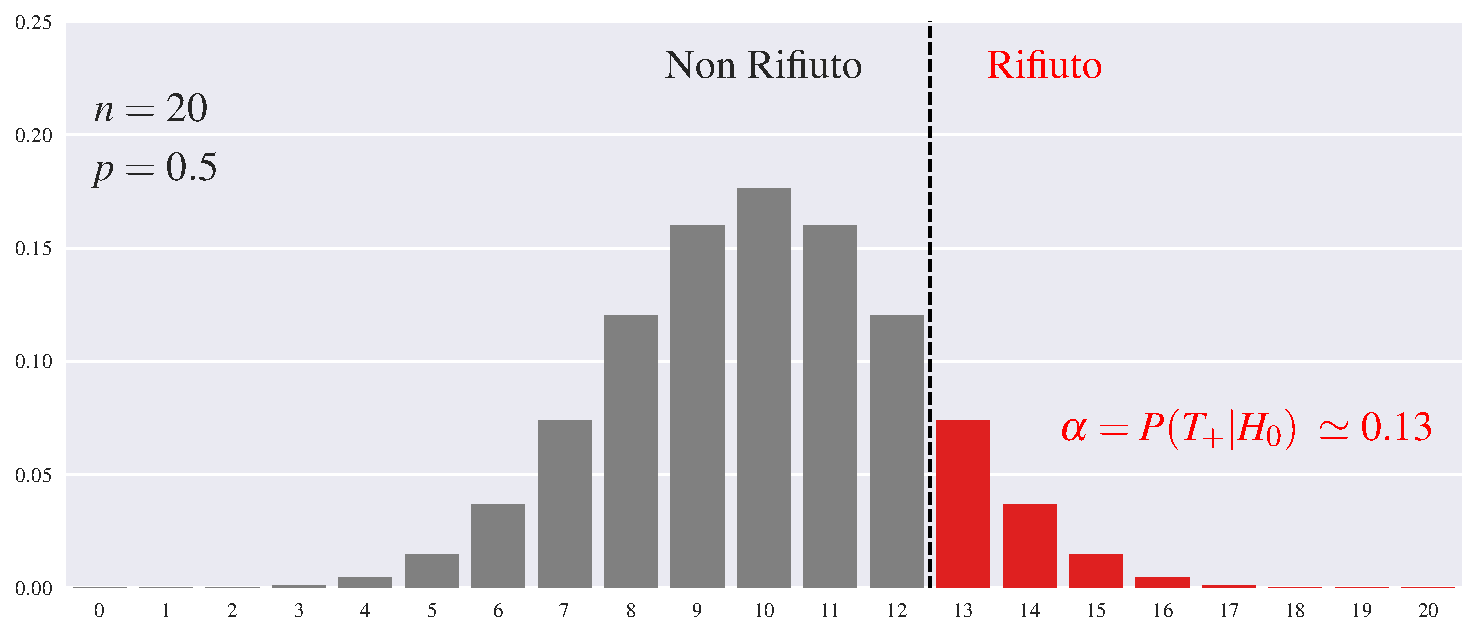
\includegraphics[width=0.9\textwidth]{figure/B-test_01.pdf}


%%%%%%%%%%%%
%%%%%%%%%%%%
%%%%%%%%%%%%
\clearpage\section{Bernoulli test (a  una coda). Errore II tipo.}

La probabilità dei falsi negativi può essere espressa in funzione di $p$ (abbiamo solo assunto che $>1/2$)


\ceq{\hfill P(T_-|D)}{=}{\sum^{k-1}_{i=1} {n\choose i}p^i(1-p)^{n-i}}

Se segliamo come prima $n=20$, $k=13$ abbiamo {\color{blue}\boldmath\ $T_-=\{0,\dots,12\}$} è la \emph{zona di NON rifiuto}.
Ora, per semplificare la discussione supponiamo di conoscere non solo il tipo ma anche la gravità del difetto. Quindi l'ipotesi alternativa diventa

$\HA:$ $p=3/4$

Rappresentiamo la distribuzione di $X$ nel caso in cui l'ipotesi alterntiva è vera. Per confronto lo accostiamo al grafico del paragrafo precedente. 


\hfil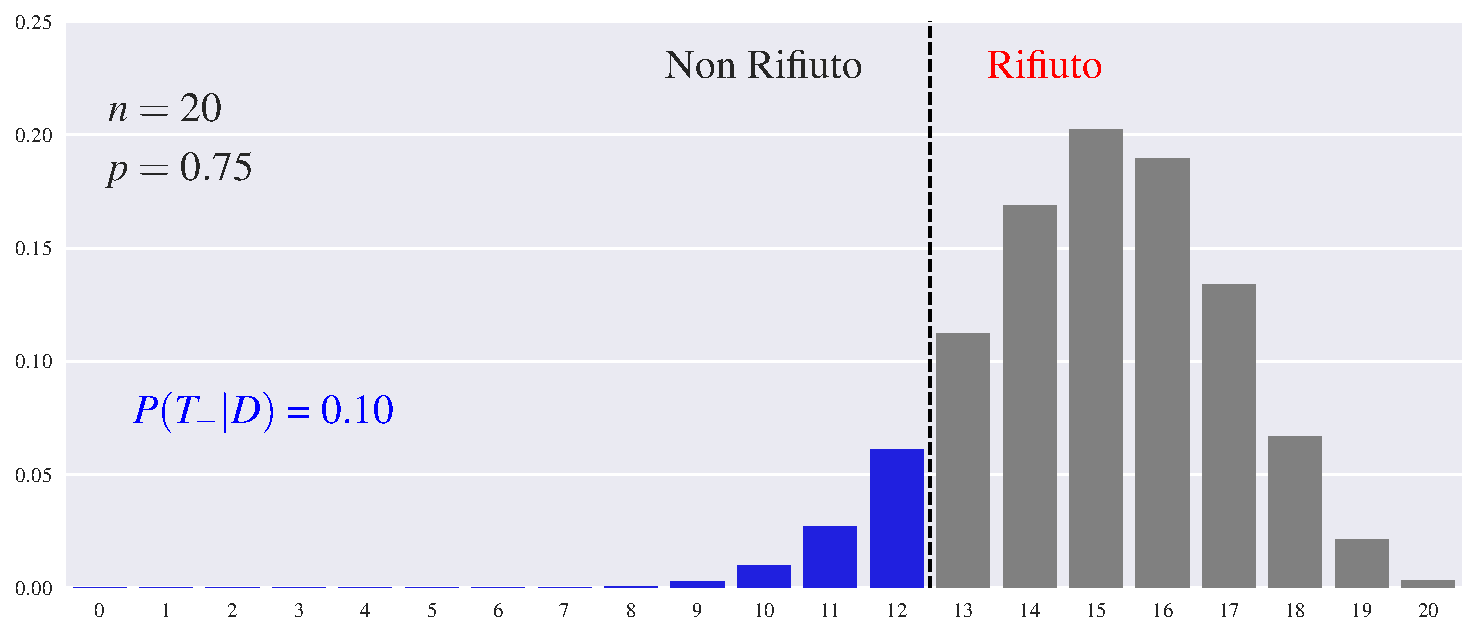
\includegraphics[width=0.9\textwidth]{figure/B-test_02.pdf}

\hfil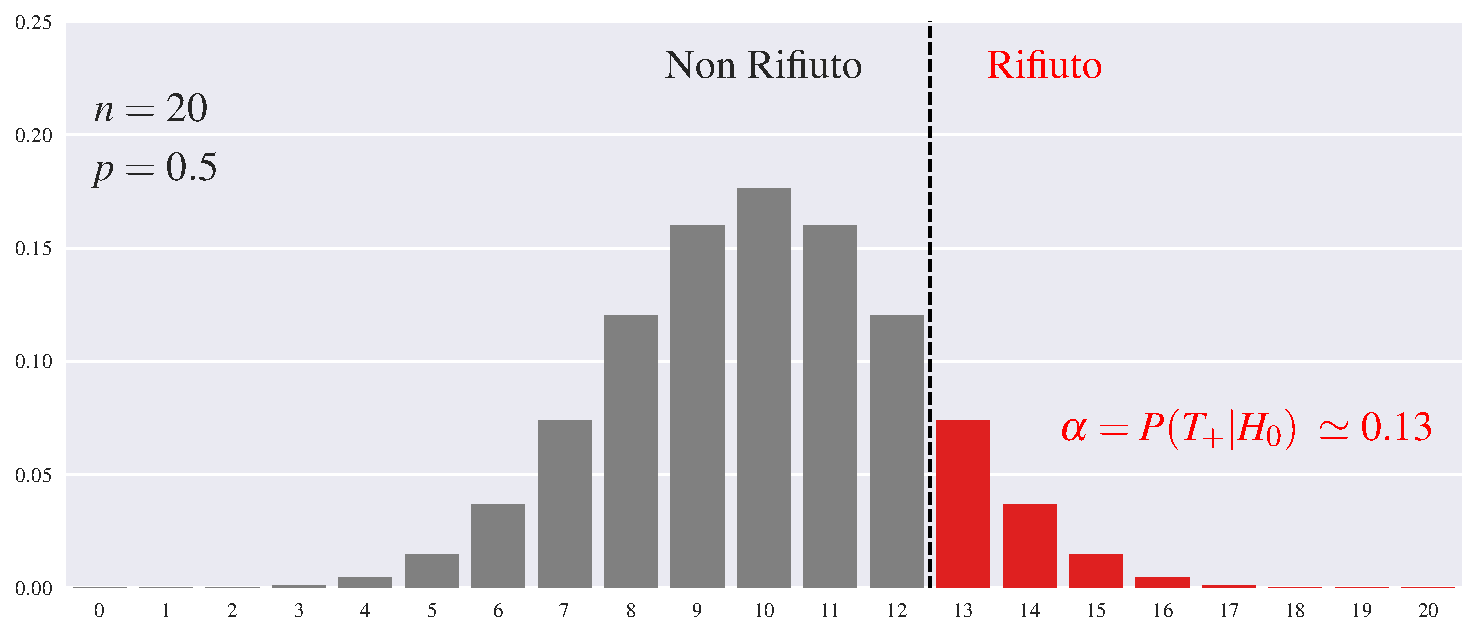
\includegraphics[width=0.9\textwidth]{figure/B-test_01.pdf}

Cosa possiamo dire sul caso generale $\HA:$ $p>1/2$~?

Al crescere di $p$ la distribuzione si sposta verso destra quindi gli errori del II tipo diminuiscono. Di converso, se $p$ si avvicina a $1/2$ l'errore aumenta al limite quando $p\approx 1/2$ avremo $\alpha+\beta\approx 1$.  


%%%%%%%%%%%%
%%%%%%%%%%%%
%%%%%%%%%%%%
\clearpage\section{Bernoulli test (due code).}

Nell'esempio precedente avevamo un'informazione certa sul tipo di difetto delle monete: sapevamo che $p>1/2$. Supponiamo questa manchi. Avremo quindi

$\H0:$ $p=1/2$

$\HA:$ $p\neq1/2$

Verifichiamo prima che il test discusso nei paragrafi precedenti \textbf{NON è adatto\/} alla nuova situazione. L'analisi di $P(T_+|\neg D)$ rimane invariata (inaftti l'insieme $\neg D$ non è cambiato).

Per semplificare la discussione dell'errore dell'secondo supponiamo per il momento che 

$\HA:$ $p=3/4$\quad o\quad $p=1/4$ 

Possiamo immaginare $D=D_{1/4}\cup D_{3/4}$. Il grafico del paragrafo precedente è valido ora se sostituiamo $D$ con $D_{3/4}$. Ora però dobbiamo considerare il caso il cui la moneta appartenga all'insieme $D_{1/4}$

\hfil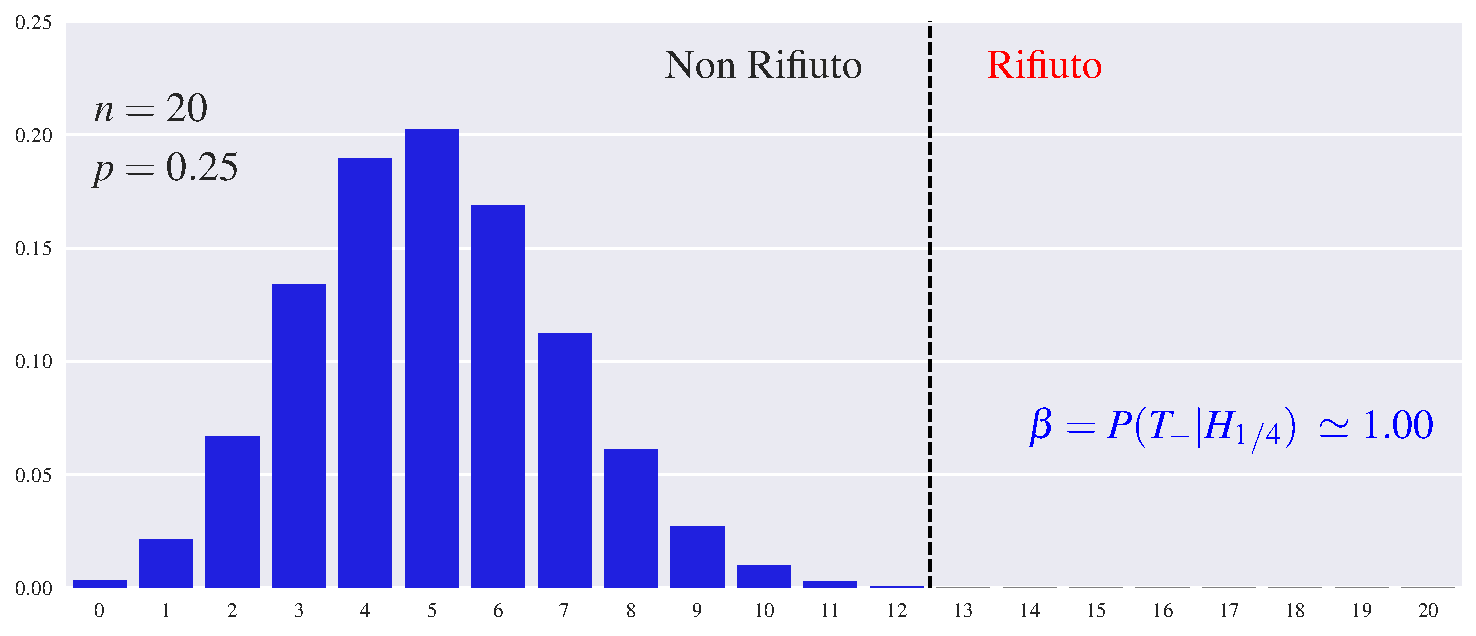
\includegraphics[width=0.9\textwidth]{figure/B-test_03.pdf}


%%%%%%%%%%%%
%%%%%%%%%%%%
%%%%%%%%%%%%
\clearpage\section{Bernoulli test (due code). Errori I e II tipo.}

Supponiamo di scegliere come zona di rifiuto $T_+=\{0,\dots,7\}\cup \{13,\dots,20\}$

\hfil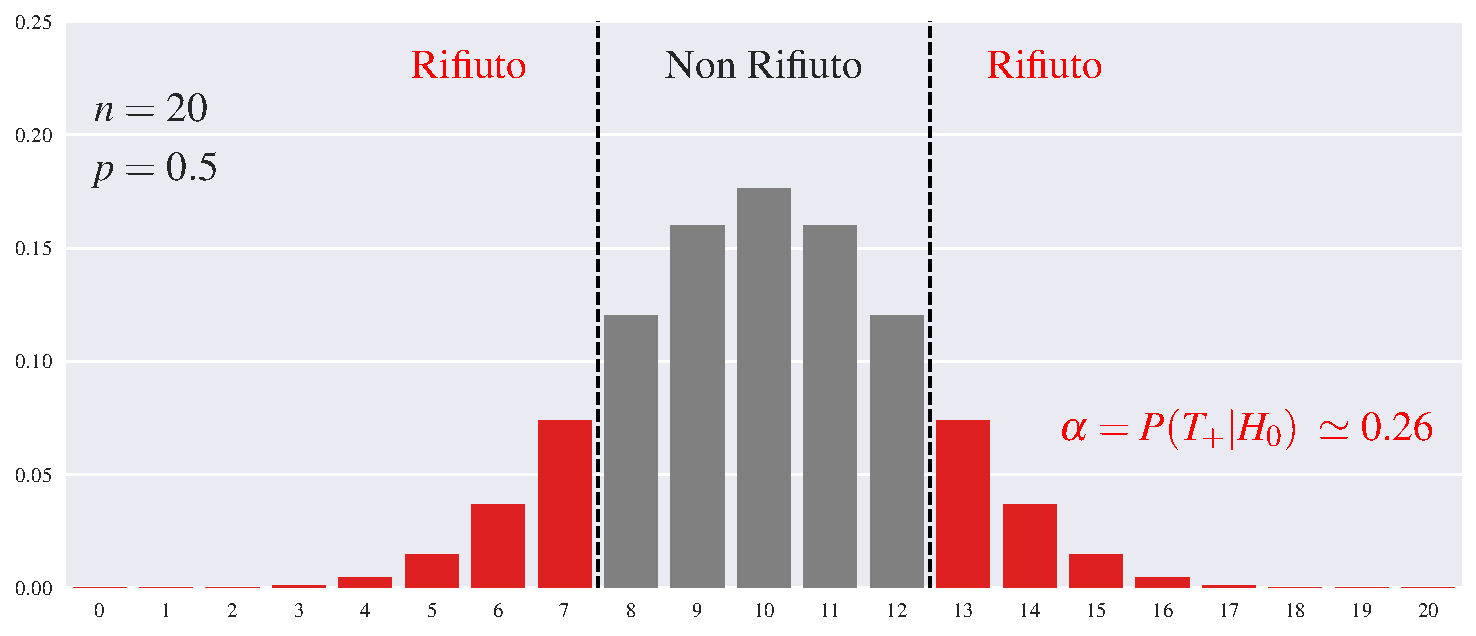
\includegraphics[width=0.9\textwidth]{figure/B-test_04.pdf}

\hfil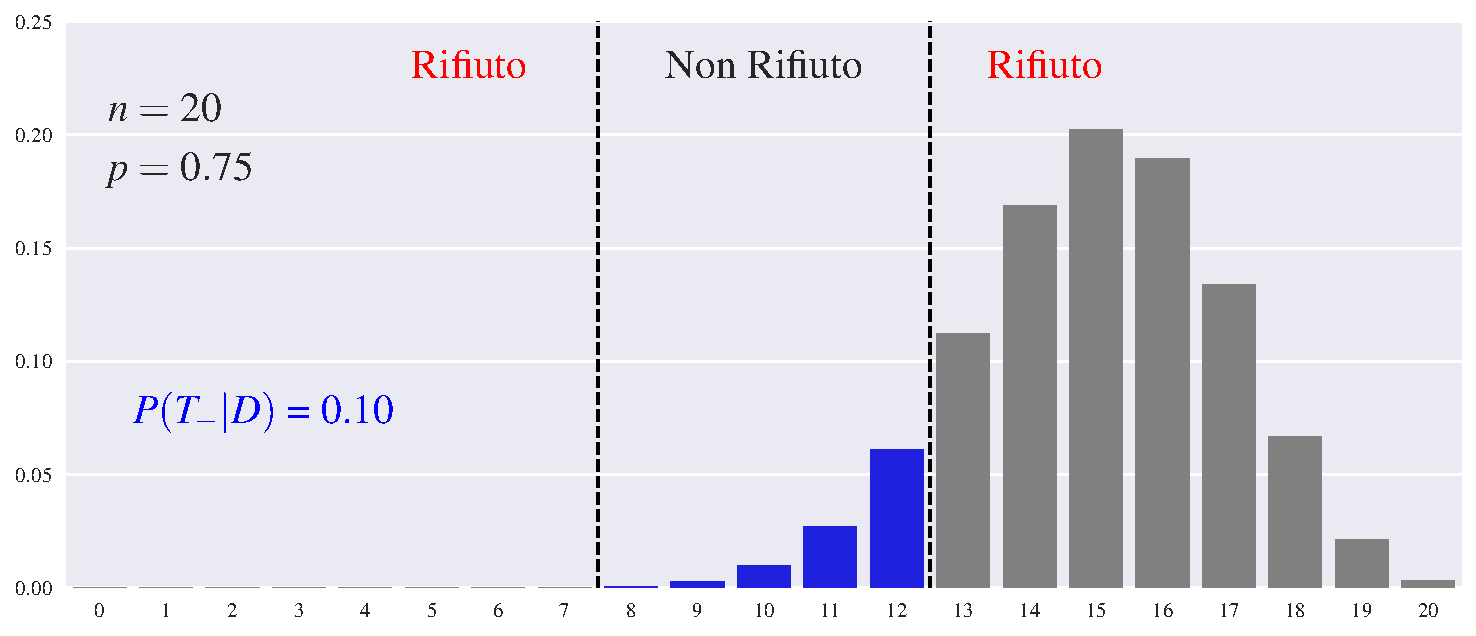
\includegraphics[width=0.9\textwidth]{figure/B-test_05.pdf}

\hfil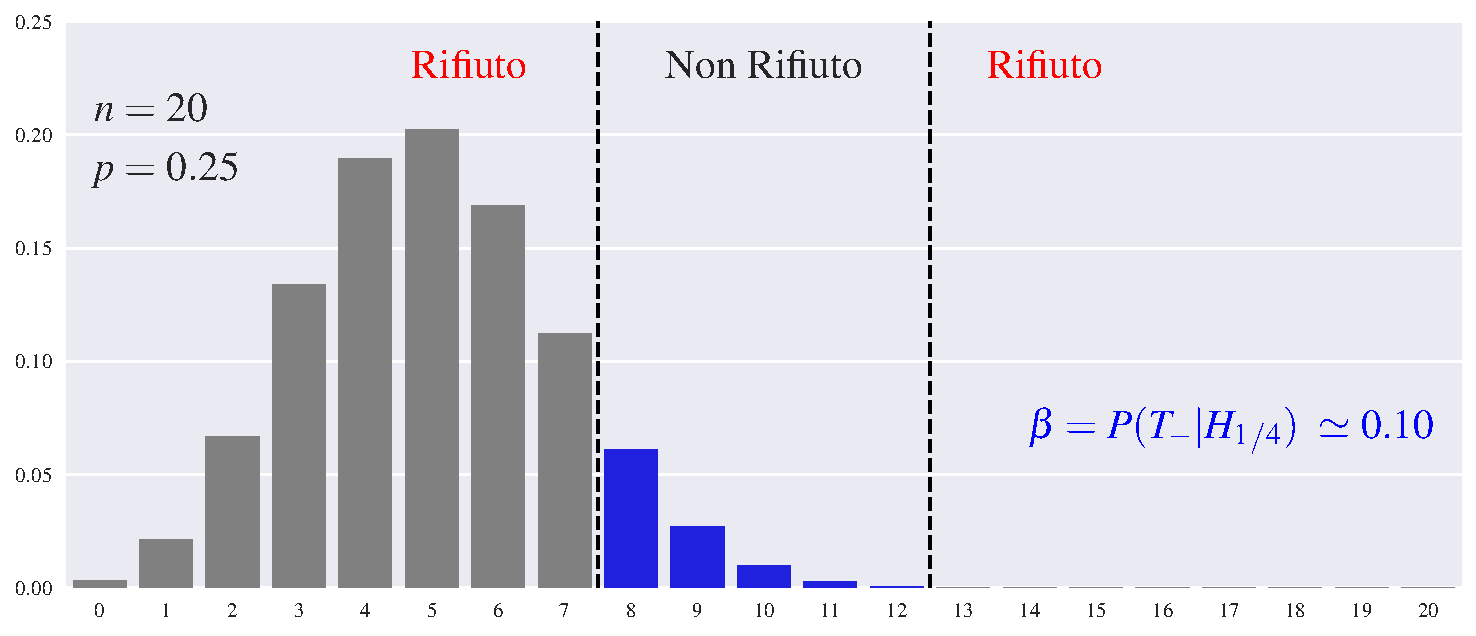
\includegraphics[width=0.9\textwidth]{figure/B-test_06.pdf}





%%%%%%%%%%%%
%%%%%%%%%%%%
%%%%%%%%%%%%
\clearpage\section{Bernoulli test (due code) campione più ampio.}

Supponiamo di raddoppiare la dimensione del campione ($n=40$). Aggiustiamo la zona di rifiuto allo stesso modo ($k=26$):  $T_+=\{0,\dots,14\}\cup \{26,\dots,40\}$

Entrambi gli errori diminuiscono.


\hfil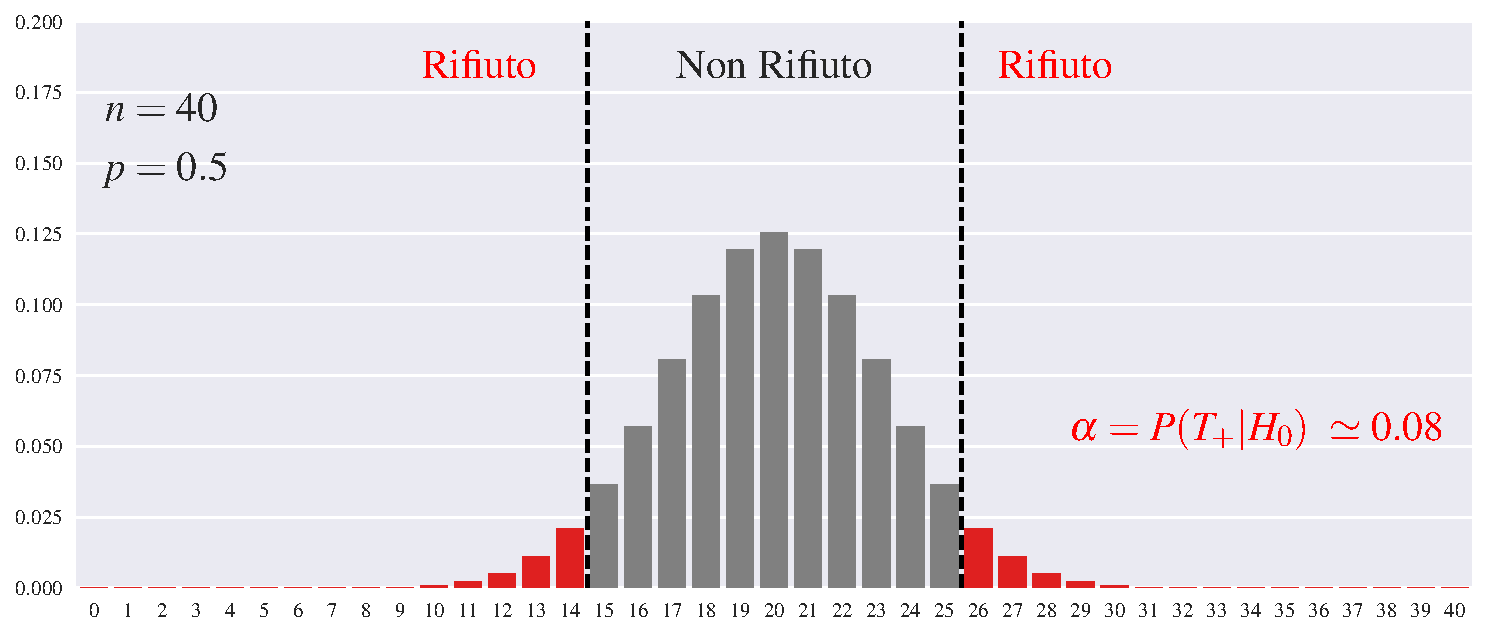
\includegraphics[width=0.9\textwidth]{figure/B-test_07.pdf}

\hfil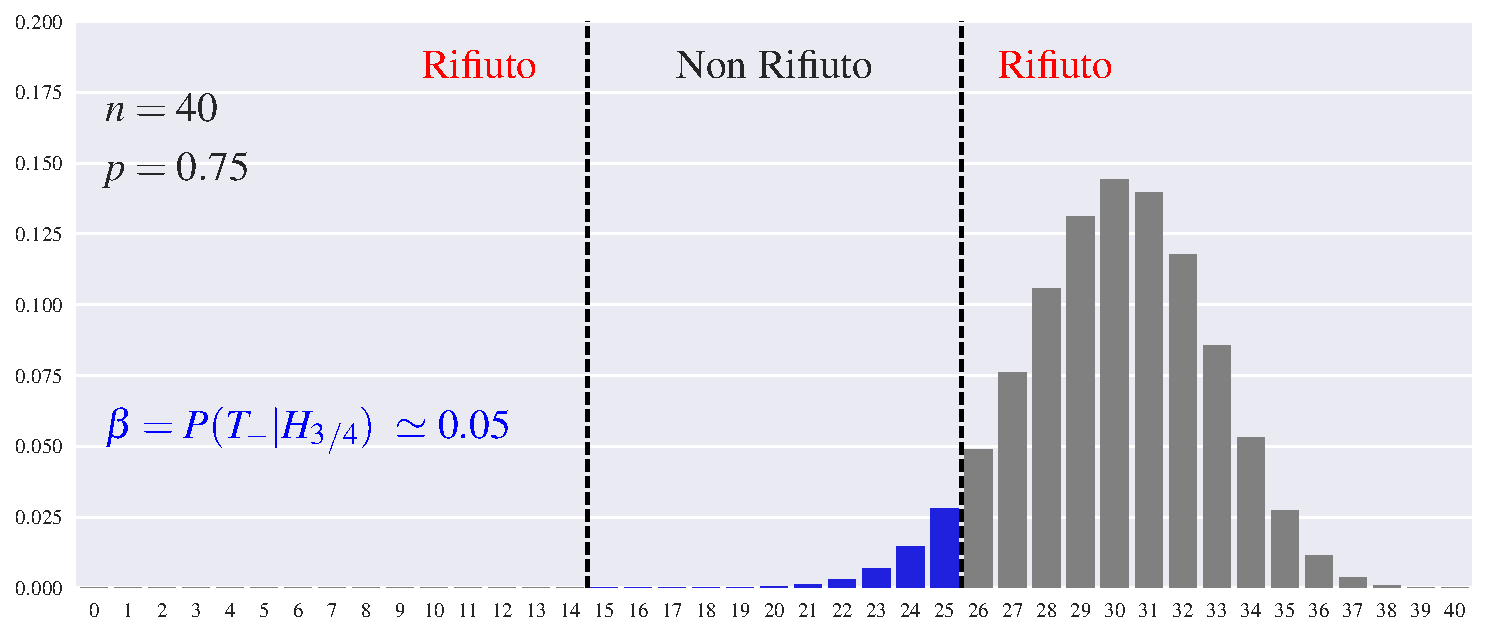
\includegraphics[width=0.9\textwidth]{figure/B-test_08.pdf}

\hfil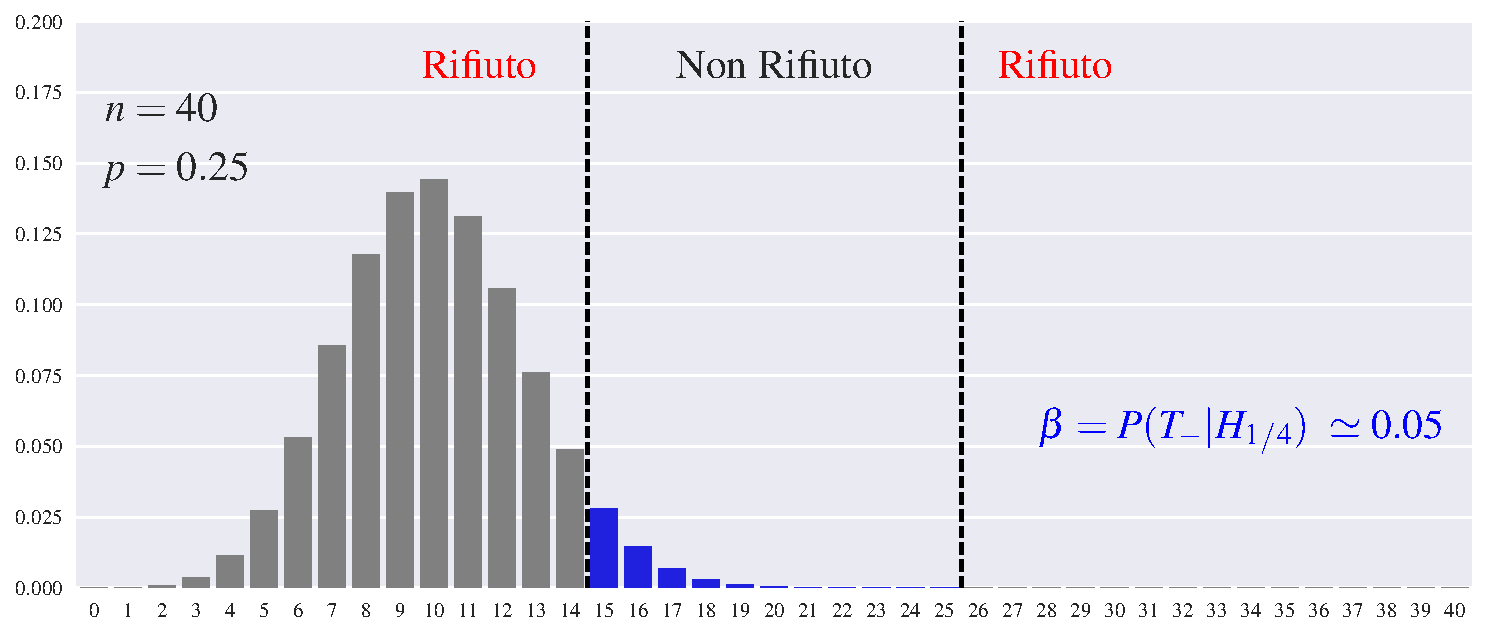
\includegraphics[width=0.9\textwidth]{figure/B-test_09.pdf}



%%%%%%%%%%%%
%%%%%%%%%%%%
%%%%%%%%%%%%
\clearpage\section{Z-test (una coda).}

(N.B. Il seguente non descrive una corretta procedura per un test clinico, cfr.\@ \hyperref[Z-test differenze (una coda)]{Z-test differenze \faShare}.) Si sospetta che una certo farmaco faccia aumentare la pressione diastolica. Nella popolazione generale la pressione diastolica nella popolazione adulta ha distribuzione $N(\mu_0,\sigma^2)$ con $\mu_0=75$ e $\sigma=9.5$. 

Assumiamo che tra i pazienti che prendono il farmaco la pressione diastolica sia distribuita normalmente con media ignota $\mu$ e con la stessa deviazione standard della popolazione generale.

Vogliamo testare le seguenti ipotesi:

$\H0:$ $\mu_0=\mu$

$\HA:$ $\mu_0>\mu$

Misurando la pressione ad un gruppo di $n$ pazienti che assumono il farmaco otteniamo un valore di $\bar x=81$ e vogliamo sapere se questo è sufficiente per rigettare $H0$.


%%%%%%%%%%%%
%%%%%%%%%%%%
%%%%%%%%%%%%
\clearpage\section{Z-test (una coda).}






\end{document}
